\section{Detailed Experiments}
\subsection{Operations}
\subsubsection*{Linear Probing}
\begin{figure}[H]
	\centering
	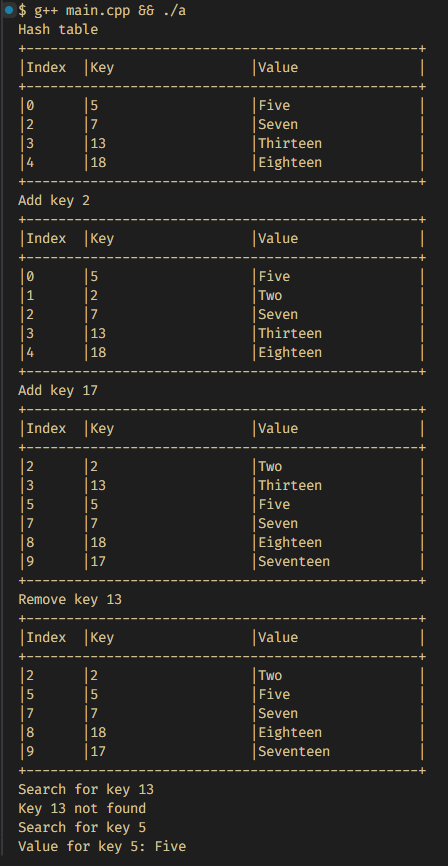
\includegraphics[width=0.5\textwidth, height=0.65\textheight]{images/linear_prob/main.png}
	\caption{Linear Probing Operations}
\end{figure}
\textbf{The hash table is initialized with size 5. Then, the following operations are performed:}
\begin{itemize}
	\item First, four keys \{7, 13, 5, 18\} are inserted to the hash table respectively.
	\item Then, key 2 is inserted (so the hash table becomes full).
	\item Continue inserting key 17 into the hash table (now the hash table needs to be rehashed to add key 17 successfully, and the indices have been changed).
	\item After that, key 13 is removed from the hash table.
	\item Therefore, when performing the search operation for key 13, it is not found in the hash table.
	\item However, key 5 is found in the hash table.
	\item Finally, the hash table is released and the program is terminated.
\end{itemize}

\subsubsection*{Quadratic Probing}
\begin{figure}[H]
	\centering
	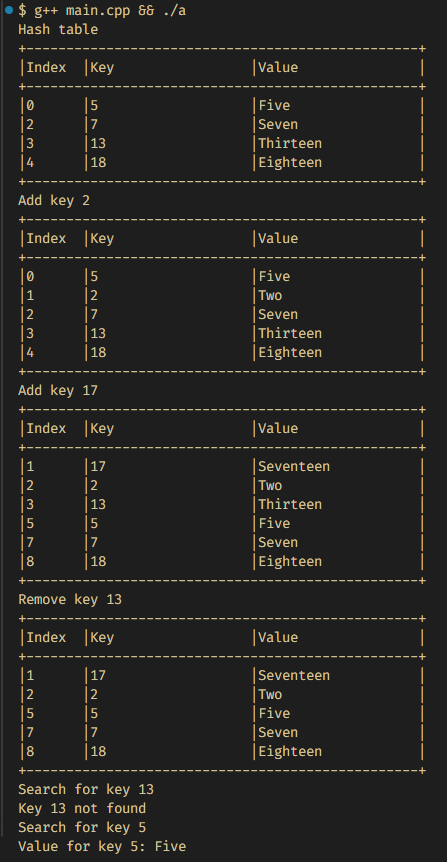
\includegraphics[width=0.5\textwidth, height=0.65\textheight]{images/quadratic_prob/main.png}
	\caption{Quadratic Probing Operations}
\end{figure}
\textbf{The hash table is initialized with size 5. Then, the following operations are performed:}
\begin{itemize}
	\item First, four keys \{7, 13, 5, 18\} are inserted to the hash table respectively.
	\item Then, key 2 is inserted (so the hash table becomes full).
	\item Continue inserting key 17 into the hash table (now the hash table needs to be rehashed to add key 17 successfully, and the indices have been changed).
	\item After that, key 13 is removed from the hash table.
	\item Therefore, when performing the search operation for key 13, it is not found in the hash table.
	\item However, key 5 is found in the hash table.
	\item Finally, the hash table is released and the program is terminated.
\end{itemize}

\subsubsection*{Chaining using Linked List}
\begin{figure}[H]
	\centering
	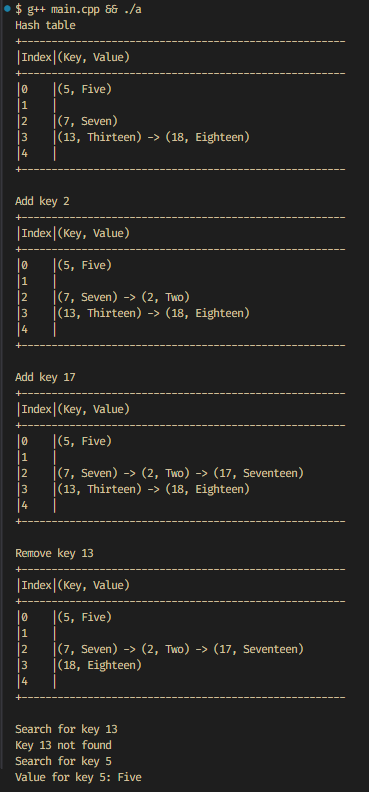
\includegraphics[width=0.5\textwidth, height=0.65\textheight]{images/chaining_ll/main.png}
	\caption{Chaining using Linked List Operations}
\end{figure}
\textbf{The hash table is initialized with size 5. Then, the following operations are performed:}
\begin{itemize}
	\item First, four keys \{7, 13, 5, 18\} are inserted to the hash table respectively.
	\item Then, key 2 and 7 are inserted.
	\item After that, key 13 is removed from the hash table.
	\item Therefore, when performing the search operation for key 13, it is not found in the hash table.
	\item However, key 5 is found in the hash table.
	\item Finally, the hash table is released and the program is terminated.
\end{itemize}

\subsubsection*{Chaining using AVL Tree}
\begin{figure}[H]
	\centering
	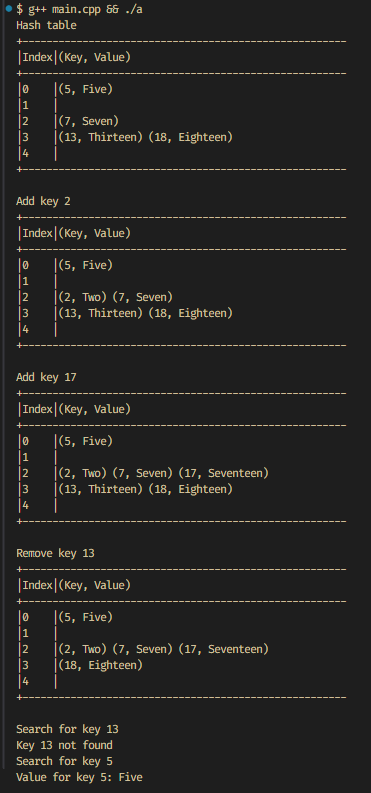
\includegraphics[width=0.5\textwidth, height=0.65\textheight]{images/chaining_avl/main.png}
	\caption{Chaining using AVL Tree Operations}
\end{figure}
\textbf{The hash table is initialized with size 5. Then, the following operations are performed:}
\begin{itemize}
	\item First, four keys \{7, 13, 5, 18\} are inserted to the hash table respectively.
	\item Then, key 2 and 7 are inserted.
	\item After that, key 13 is removed from the hash table.
	\item Therefore, when performing the search operation for key 13, it is not found in the hash table.
	\item However, key 5 is found in the hash table.
	\item Finally, the hash table is released and the program is terminated.
\end{itemize}

\subsubsection*{Double Hashing}
\begin{figure}[H]
	\centering
	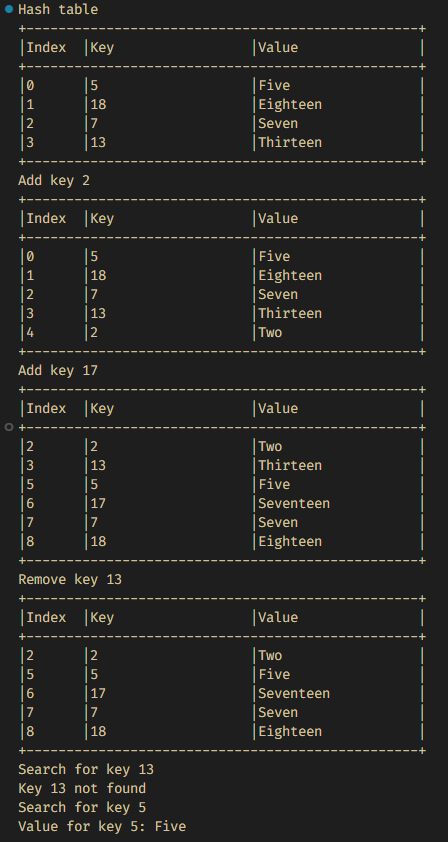
\includegraphics[width=0.5\textwidth, height=0.65\textheight]{images/double_hash/main.png}
	\caption{Double Hashing Operations}
\end{figure}
\textbf{The hash table is initialized with size 5. Then, the following operations are performed:}
\begin{itemize}
	\item First, four keys \{7, 13, 5, 18\} are inserted to the hash table respectively.
	\item Then, key 2 is inserted (so the hash table becomes full).
	\item Continue inserting key 17 into the hash table (now the hash table needs to be rehashed to add key 17 successfully, and the indices have been changed).
	\item After that, key 13 is removed from the hash table.
	\item Therefore, when performing the search operation for key 13, it is not found in the hash table.
	\item However, key 5 is found in the hash table.
	\item Finally, the hash table is released and the program is terminated.
\end{itemize}

\subsection{Performance}
\subsubsection*{Linear Probing}
\begin{figure}[H]
	\centering
	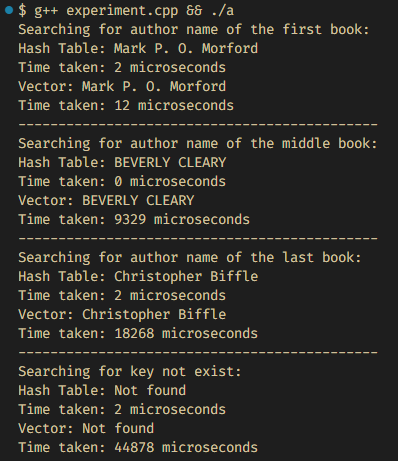
\includegraphics[width=0.6\textwidth]{images/linear_prob/experiment.png}
	\caption{Linear Probing Performance}
\end{figure}
\begin{itemize}
	\item Time Complexity of Linear Probing Search: \(O(n)\)
	\item Time Complexity of Linear Seach Algorithm: \(O(n)\)
\end{itemize}
Though having the same theorectical time complexity, the actual time execution of Linear Probing Search is much faster than Linear Search Algorithm, especially in the worst case.

\subsubsection*{Quadratic Probing}
\begin{figure}[H]
	\centering
	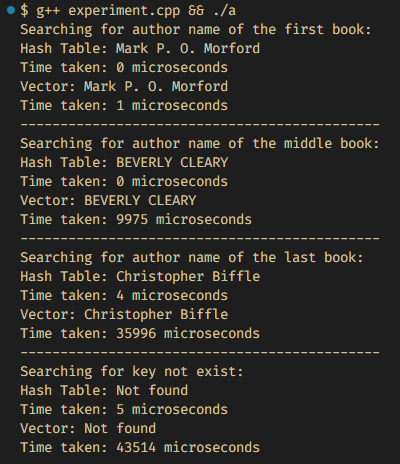
\includegraphics[width=0.6\textwidth]{images/quadratic_prob/experiment.png}
	\caption{Quadratic Probing Performance}
\end{figure}
\begin{itemize}
	\item Time Complexity of Quadratic Probing Search: \(O(n)\)
	\item Time Complexity of Linear Seach Algorithm: \(O(n)\)
\end{itemize}
Though having the same theorectical time complexity, the actual time execution of Quadratic Probing Search is much faster than Linear Search Algorithm, especially in the worst case.

\subsubsection*{Chaining using Linked List}
\begin{figure}[H]
	\centering
	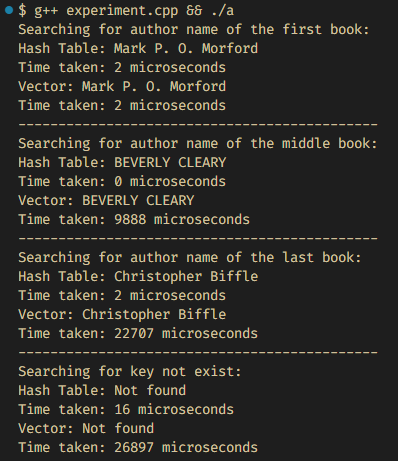
\includegraphics[width=0.6\textwidth]{images/chaining_ll/experiment.png}
	\caption{Chaining using Linked List Performance}
\end{figure}
\begin{itemize}
	\item Time Complexity of Chaining Search using Linked List: \(O(n)\)
	\item Time Complexity of Linear Seach Algorithm: \(O(n)\)
\end{itemize}
Though having the same theorectical time complexity, the actual time execution of Chaining Search using Linked List is much faster than Linear Search Algorithm, especially in the worst case.

\subsubsection*{Chaining using AVL Tree}
\begin{figure}[H]
	\centering
	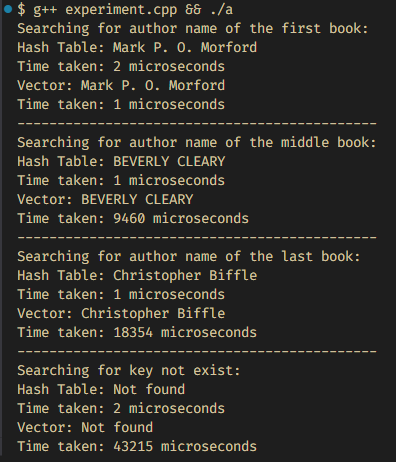
\includegraphics[width=0.6\textwidth]{images/chaining_avl/experiment.png}
	\caption{Chaining using AVL Tree Performance}
\end{figure}
\begin{itemize}
	\item Time Complexity of Chaining Search using AVL Tree: \(O(\log n)\)
	\item Time Complexity of Linear Seach Algorithm: \(O(n)\)
\end{itemize}
Chaining Search using AVL Tree has a better time complexity than Linear Search Algorithm in theorectical, and the actual time also proves that.

\subsubsection*{Double Hashing}
\begin{figure}[H]
	\centering
	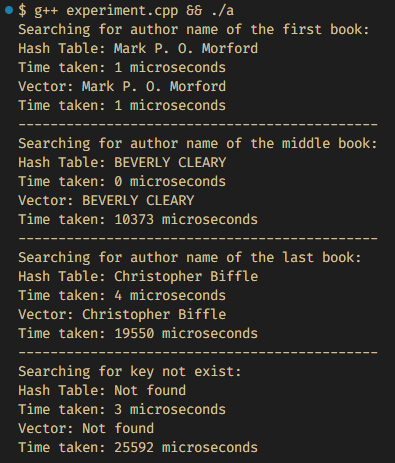
\includegraphics[width=0.6\textwidth]{images/double_hash/experiment.png}
	\caption{Double Hashing Performance}
\end{figure}
\begin{itemize}
	\item Time Complexity of Double Hashing Search: \(O(n)\)
	\item Time Complexity of Linear Seach Algorithm: \(O(n)\)
\end{itemize}
Though having the same theorectical time complexity, the actual time execution of Double Hashing Search is much faster than Linear Search Algorithm, especially in the worst case.
